\section{AdaBoost}

O modelo \textit{boosting} refere-se a um método \textit{ensemble} (sessão \ref{sec:ensemble}) para resolver problemas de classificação e regressão. A ideia geral do \textit{boosting} é  combinar vários algoritmos fracos em um modelo robusto. Esses algoritmos são treinados em sequência, onde cada um tenta corrigir seu antecessor \cite{Kearns:1988}.

O algoritmo do tipo \textit{boosting} mais conhecido na literatura é o \textit{Adaptive Boosting} ou simplesmente \textit{AdaBoost}, que foi proposto por \cite{Freund:1997}. O algoritmo pode ser usado para melhorar o desempenho de qualquer algoritmo de \textit{machine learning}. Contudo, AdaBoost funciona melhor com preditores fracos \footnote{Preditores fracos são aqueles que alcançam uma acurácia pouco acima de um preditor aleatório.}.

O preditor mais comum para ser usado com o AdaBoost são as árvores de decisão com um nível. Pelo fato dessas árvores possuírem apenas um nível, são conhecidas na literatura como \textit{Decision Stump} (algo como Toco de Decisão, em vez de Árvore de Decisão).

\subsection{Funcionamento}
O trabalho de \cite{Freund:1999} foi utilizado como referência para a explicação do funcionamento do algoritmo que será dada a seguir.

Inicialmente, é fornecido como entrada para o algoritmo, o conjunto de treino $(x_1, y_1), (x_2, y_2) ..., (x_m, y_m)$, onde cada $x_i$ pertence ao conjunto de instâncias $X$, e cada $y_i$ pertence ao conjunto de rótulos $Y$. Para problemas envolvendo a classificação binária (ou dicotômica), considera-se $Y = \{-1, +1\}$. 

Adaboost utiliza $T$ preditores, os autores chamam os preditores de \textit{hipóteses}, denotando as hipóteses como sendo $h_1(x), h_2(x),..., h_T(x)$, onde $x$ representa uma instância a ser classificada pela hipótese $h_t(x)$.

Uma das principais ideias do algoritmo é manter um conjunto de
pesos sobre o conjunto de treinamento. Isto é, para cada instância no conjunto de treinamento há um peso associado e, a medida que o algoritmo evolui, quanto mais difícil for para classificar uma instância de treinamento, maior será o peso atribuído a ela. De modo que, para os preditores subsequentes, a chance de classificar corretamente esse dado é maior. O peso dessa distribuição para um dado de treinamento $i$ na rodada $t$ é denotado por $D_t(i)$.

Inicialmente, todas as instâncias no conjunto de treinamento possuem exatamente o mesmo peso $w_i = \dfrac{1}{N}$, onde $N$ é o tamanho do conjunto de treinamento. Mas, a cada rodada, o peso das amostras classificadas erroneamente são aumentados, dessa forma, os preditores são forçados a focar nas amostras mais difíceis de serem classificadas. A cada rodada $t$ o peso de cada amostra é normalizado de acordo com o somatório de pesos de todas as amostras $Z_t = \sum_{i=1}^{N} D_t(i)$


%\begin{document}
 %Código
 \begin{algorithm}[H]
   \SetAlgoLined
   \Entrada{$(x_1, y_1), (x_2, y_2),...,(x_N, y_N)$, onde $x_i \in X$ e $y_i \in Y = \{-1, 1\}$} 
   \Saida{Classificador $H(x)$}
   
   Inicialize $D_1(i) = \frac{1}{N}$.   
   
    \Para{cada $t = 1,...,T$}{
        Treine o preditor usando a distribuição $D_t$ \\
        Calcule a taxa de erro $\epsilon_t$ \\
        Calcule o peso do preditor $ \alpha_t = \frac{1}{2} \times \frac{1-\epsilon_t}{\epsilon_t}$ \\
        Atualize os pesos dos dados $D_{t+1}(i) = \frac{D_t(i)}{Z_t} \times
        \begin{cases} 
            e^{-\alpha_t}, & \mbox{se } h_t(x_i) = y_i \\
            e^{\alpha_t}, & \mbox{se } h_t(x_i) \neq y_i 
        \end{cases}$
        
    }
   
   \Retorna{$sign \begin{pmatrix} \sum_{t=1}^{T} \alpha_t h_t(x) \end{pmatrix}$}
   \label{alg:adaboost}
   \caption{\textsc{AdaBoost}}
 \end{algorithm}
%\end{document}

\begin{figure}[ht!] 
    \centering
    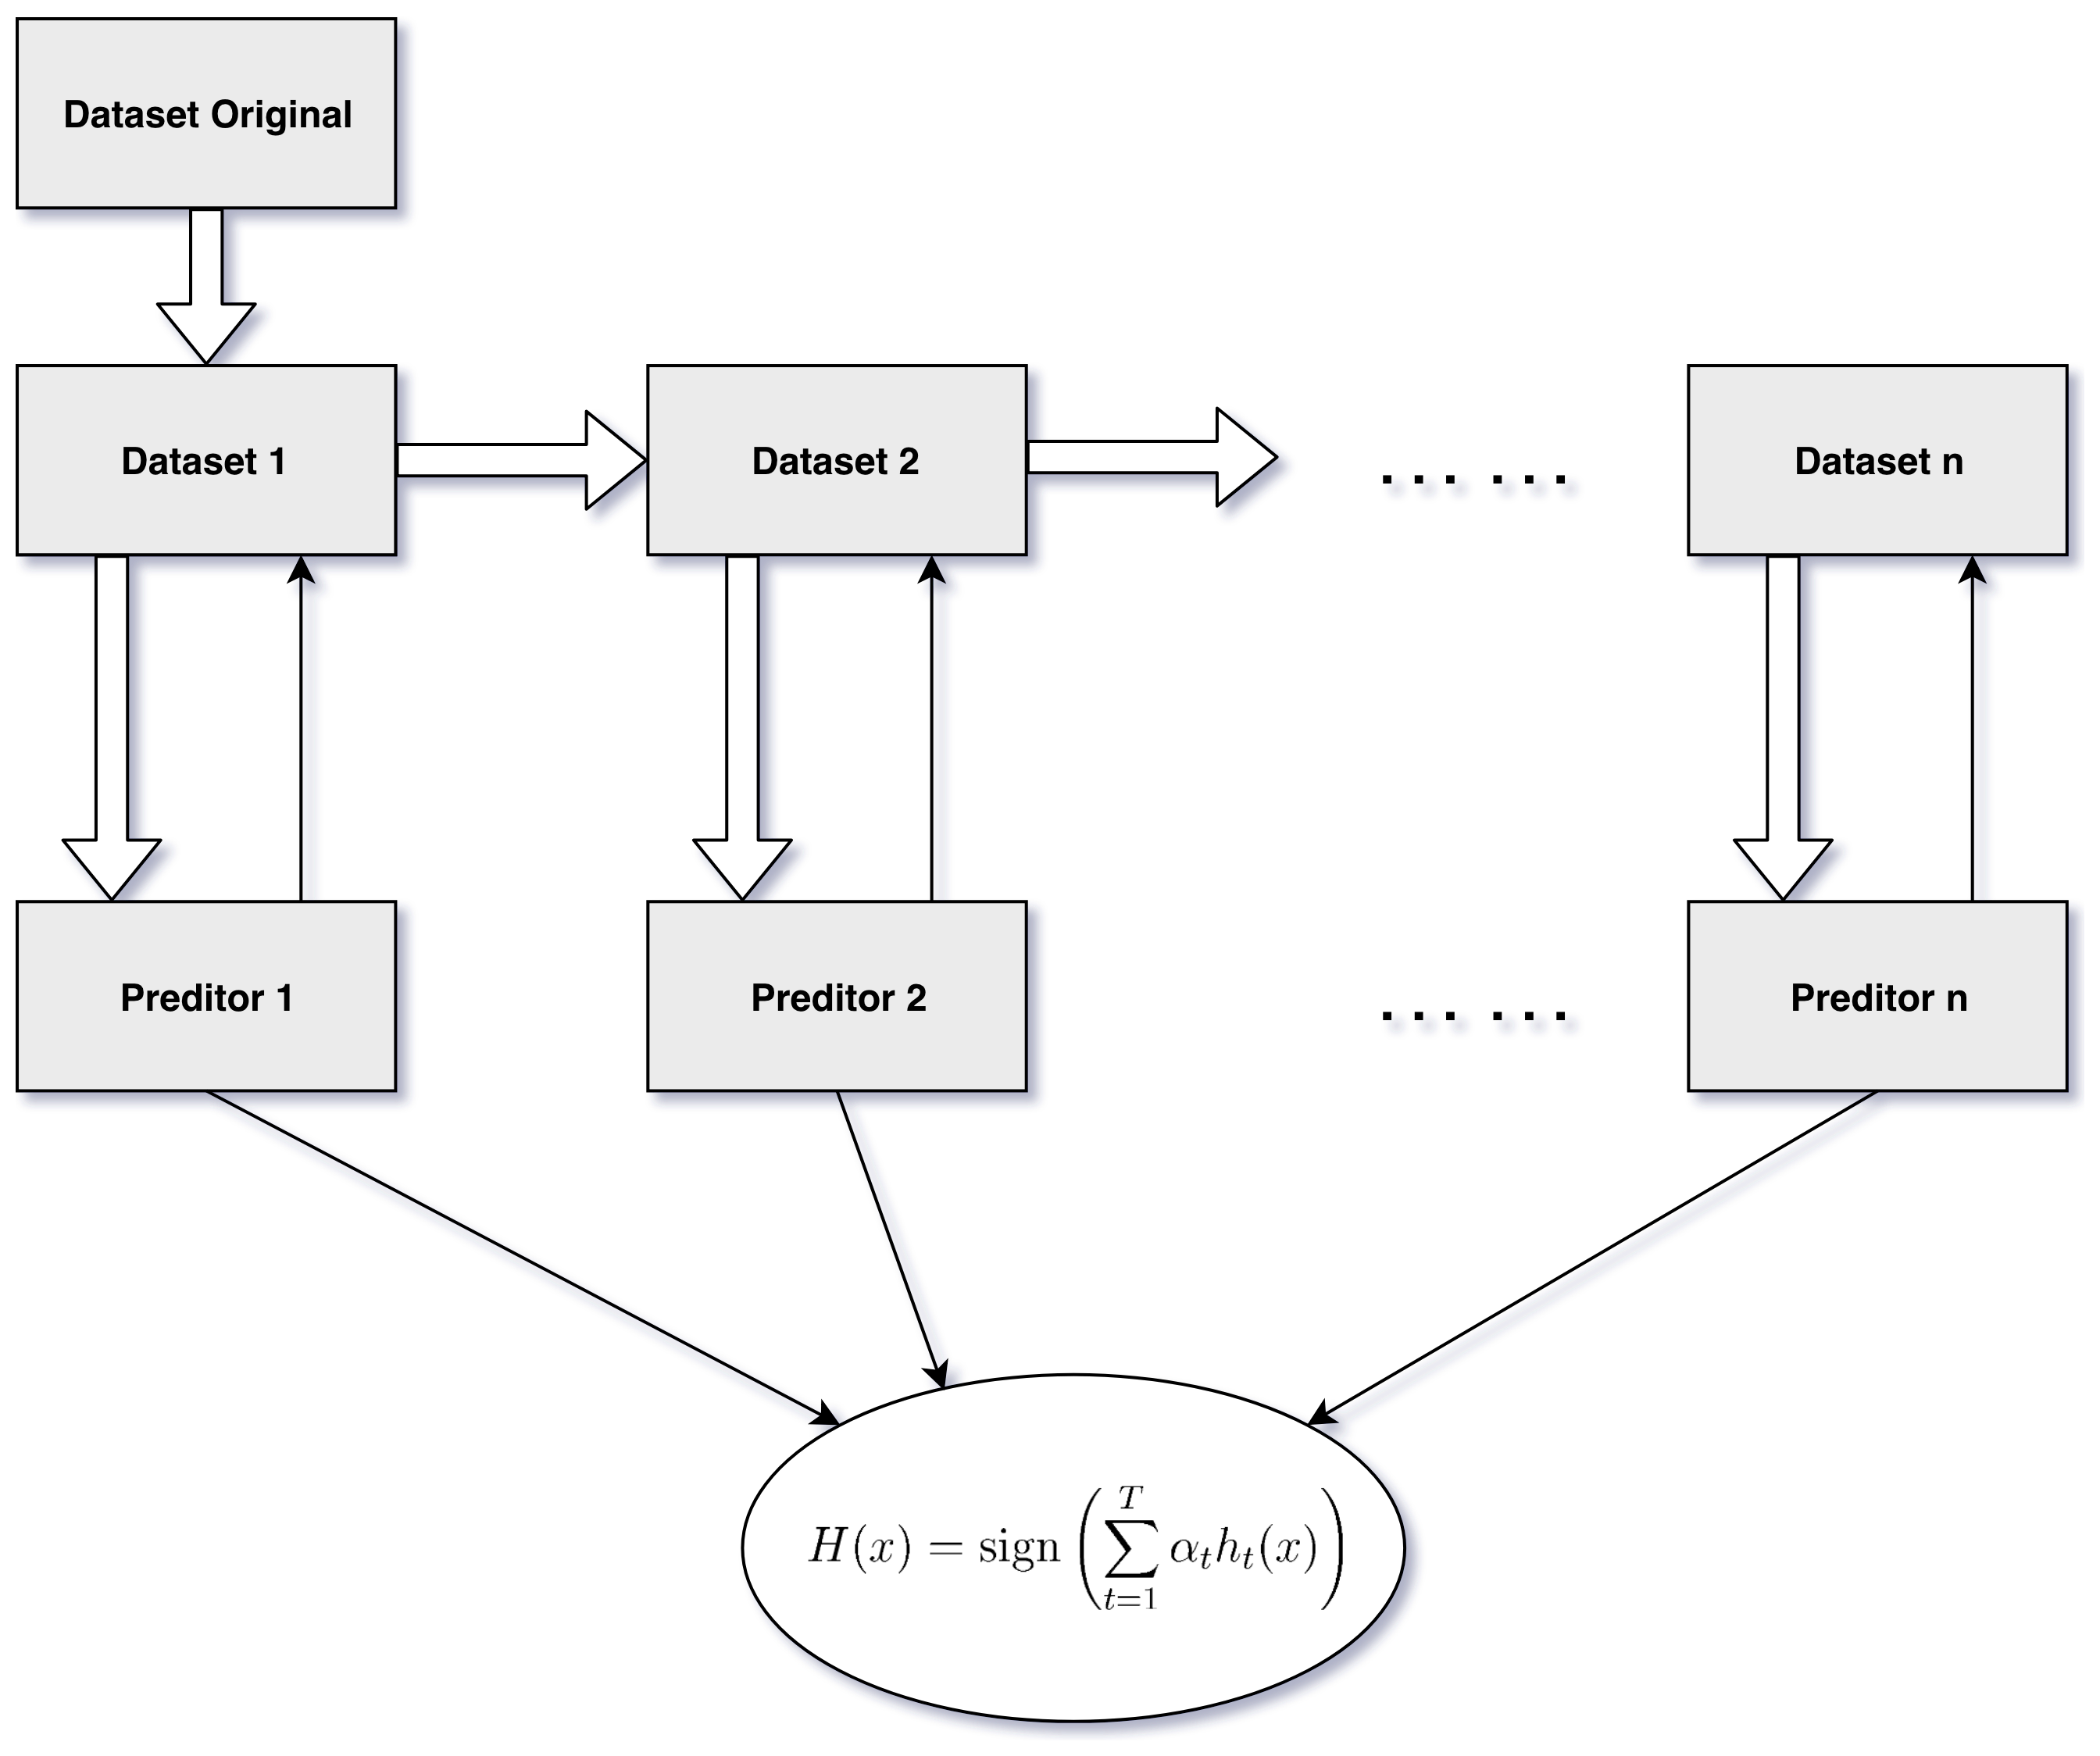
\includegraphics[scale=0.15]{Imagens/Model-Adaboost.png}
    \caption{Funcionamento do algoritmo AdaBoost}
    \label{fig:adaboost}
\end{figure}

A figura \ref{fig:adaboost} ilustra o funcionamento do algoritmo AdaBoost, percebe-se que há um encadeamento entre os preditores, além disso, percebe-se que cada preditor influencia no \textit{dataset} que será utilizado no preditor subsequente.



\subsection{Vantagens e Desvantagens}